\documentclass[article]{jss}
\usepackage[utf8]{inputenc}

\providecommand{\tightlist}{%
  \setlength{\itemsep}{0pt}\setlength{\parskip}{0pt}}

\author{
Earo Wang\\Monash University \And Dianne Cook\\Monash University \And Rob J Hyndman\\Monash University
}
\title{Calendar-based graphics for visualizing people's daily schedules}

\Plainauthor{Earo Wang, Dianne Cook, Rob J Hyndman}
\Plaintitle{Calendar-based graphics for visualizing people's daily schedules}

\Abstract{
This paper describes a \code{frame\_calendar} function that organizes
and displays temporal data, collected on sub-daily resolution, into a
calendar layout. Calendars are broadly used in society to display
temporal information, and events. The \code{frame\_calendar} utilizes
linear algebra on the date variable to create the layout. It utilizes
the grammar of graphics to create the plots inside each cell, and thus
synchronises neatly with \pkg{ggplot2} graphics. The motivating
application is studying pedestrian behavior, based on counts which are
captured at hourly intervals by sensors scattered around the city.
Faceting by the usual features such as day and month, was insufficient
to examine the behavior. Making displays on a monthly calendar format
helps to understand pedestrian patterns relative to events such as work
days, weekends, holidays, and special events. The layout algorithm has
several format options and variations. It is implemented in the R
package \pkg{sugrrants}.
}

\Keywords{data visualization, statistical graphics, time series, R package, grammar of graphics}
\Plainkeywords{data visualization, statistical graphics, time series, R package, grammar of graphics}

%% publication information
%% \Volume{50}
%% \Issue{9}
%% \Month{June}
%% \Year{2012}
%% \Submitdate{}
%% \Acceptdate{2012-06-04}

\Address{
    Earo Wang\\
  Monash University\\
  Department of Econometrics and Business Statistics, Monash University,
  VIC 3800 Australia\\
  E-mail: \email{earo.wang@monash.edu}\\
  
      Dianne Cook\\
  Monash University\\
  Department of Econometrics and Business Statistics, Monash University,
  VIC 3800 Australia\\
  E-mail: \email{dicook@monash.edu}\\
  
      Rob J Hyndman\\
  Monash University\\
  Department of Econometrics and Business Statistics, Monash University,
  VIC 3800 Australia\\
  E-mail: \email{rob.hyndman@monash.edu}\\
  
  }

% Pandoc header

\usepackage{amsmath}

\usepackage{amsthm}
\newtheorem{theorem}{Theorem}[section]
\newtheorem{lemma}{Lemma}[section]
\theoremstyle{definition}
\newtheorem{definition}{Definition}[section]
\newtheorem{corollary}{Corollary}[section]
\newtheorem{proposition}{Proposition}[section]
\theoremstyle{definition}
\newtheorem{example}{Example}[section]
\theoremstyle{remark}
\newtheorem*{remark}{Remark}
\begin{document}

\section{Introduction}\label{introduction}

We develop a method for organizing and visualizing temporal data,
collected on sub-daily interval, into a calendar layout. The purpose of
the calendar-based visualization is to provide insights into people's
daily schedules relative to events such as work days, weekends,
holidays, and special events. This work was originally motivated by
studying foot traffic in the city of Melbourne \citep{ped}. There have
been 43 sensors installed that count pedestrians every hour across the
downtown area (Figure \ref{fig:ped-map}). The dataset can shed light
into understanding people's daily rhythms, to assist the city
administration and local businesses with event planning and operational
management. A routine examination of the data would be constructing a
conventional time series plot to catch a glimpse of temporal patterns.
The facetted plots in Figure \ref{fig:time-series-plot}, give an overall
picture of the foot traffic at 3 different sensors over 2016. Further
facetting by day of the week (Figure \ref{fig:facet-time}) provides a
better glimpse at the daily and sub-daily, like commuter, patterns. The
sensor data, like many temporal datasets on human behaviors, lends
itself to a number of exploratory data visualization challenges:

\begin{enumerate}
\def\labelenumi{\arabic{enumi}.}
\tightlist
\item
  Variations primarily source from multiple time scales including time
  of day, day of week, and day of year (such as public holiday and
  recurring events).
\item
  Since the data are often collected at sub-daily frequencies, they
  typically involve a large number of observations.
\item
  Measurements of a single type are made at multiple locations at a
  given time point, which creates the need for comparing and contrasting
  between locations.
\end{enumerate}

and the conventional ways to display time series and constructing
facetted displays don't completely address these challenges.

\begin{CodeChunk}
\begin{figure}

{\centering 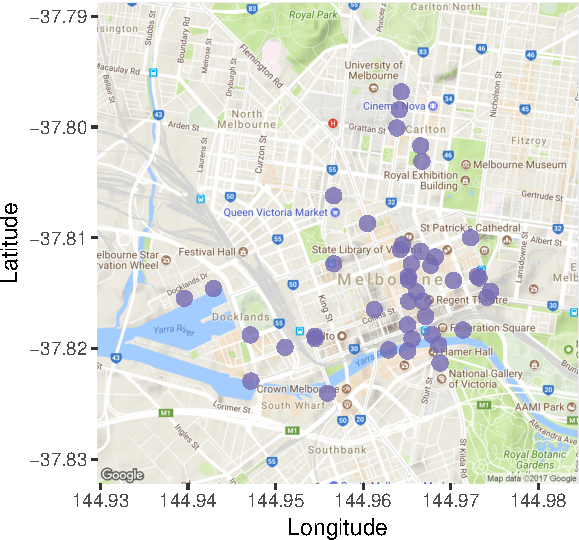
\includegraphics[width=0.55\linewidth]{figure/ped-map-1} 

}

\caption[Map of the Melbourne city with purple dots indicating
sensor locations.]{Map of the Melbourne city with purple dots indicating
sensor locations.}\label{fig:ped-map}
\end{figure}
\end{CodeChunk}




\begin{CodeChunk}
\begin{figure}

{\centering 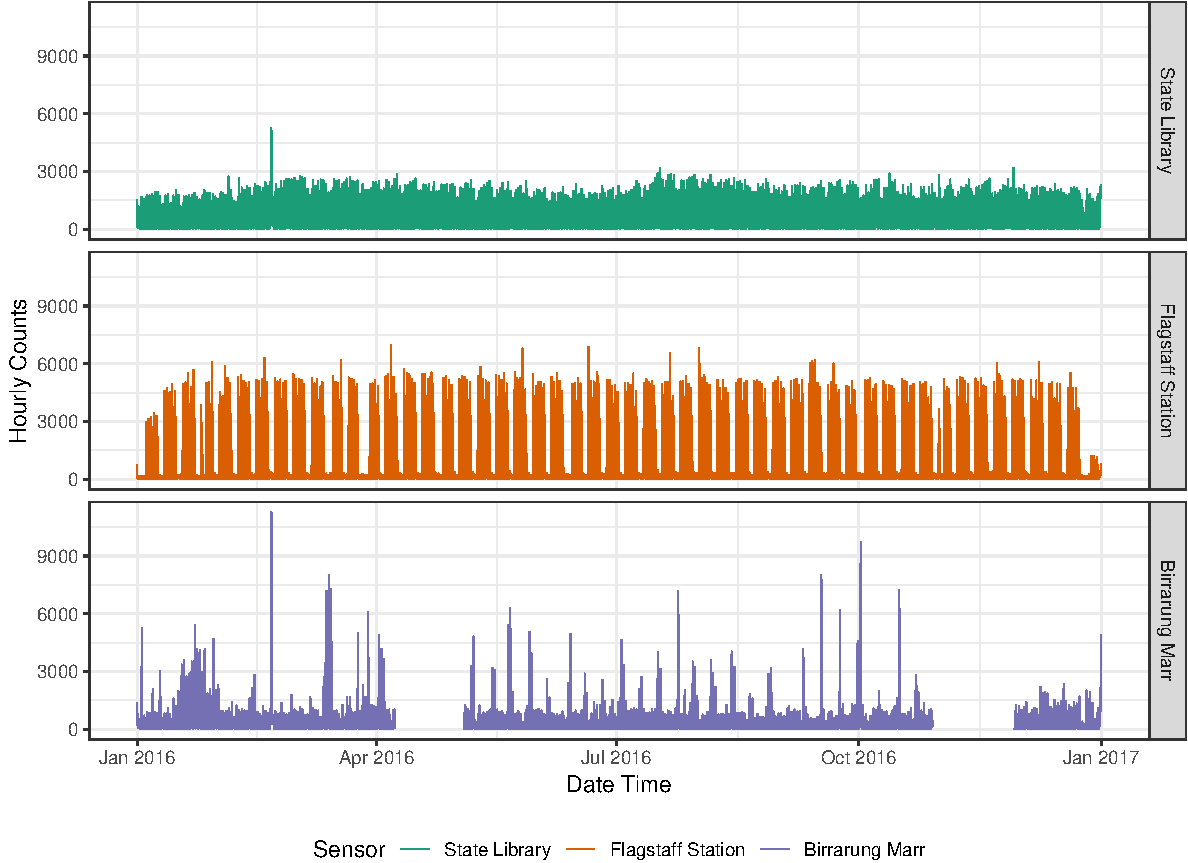
\includegraphics[width=\textwidth]{figure/time-series-plot-1} 

}

\caption[Time series plot about the number of
pedestrians in 2016 measured at 3 different sensors in the city of
Melbourne. Coloured by the sensors, small multiples of lines show that
the foot traffic varies from one sensor to another in terms of both time
and number. The weekly patterns look distinctive across these 3 sensors.
There is an eye-catching spike which occurred at State Library, caused
by the annual event--White Night--on 20th of February.]{Time series plot about the number of
pedestrians in 2016 measured at 3 different sensors in the city of
Melbourne. Coloured by the sensors, small multiples of lines show that
the foot traffic varies from one sensor to another in terms of both time
and number. The weekly patterns look distinctive across these 3 sensors.
There is an eye-catching spike which occurred at State Library, caused
by the annual event--White Night--on 20th of February.}\label{fig:time-series-plot}
\end{figure}
\end{CodeChunk}









\begin{CodeChunk}
\begin{figure}

{\centering 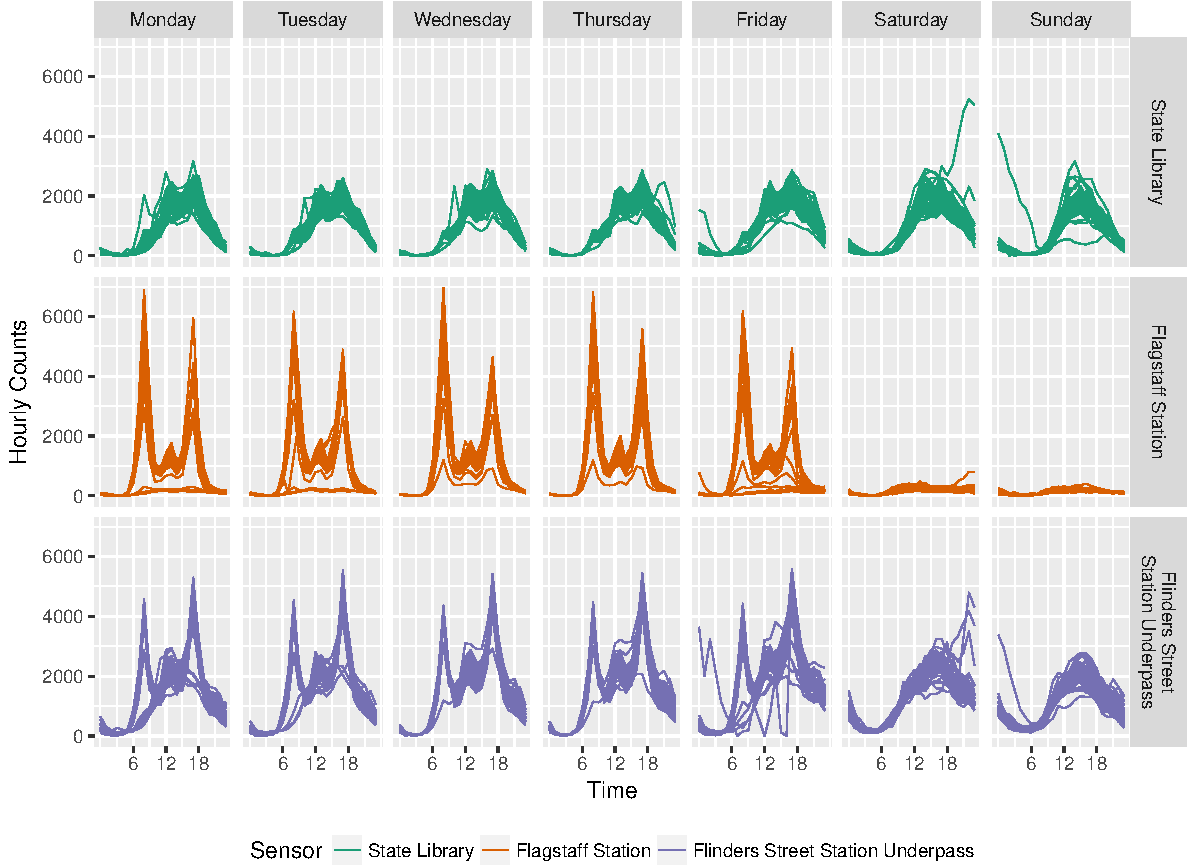
\includegraphics[width=\textwidth]{figure/facet-time-1} 

}

\caption[Hourly pedestrian counts faceted by sensors and
days of the week using lines. It features at least two types of
seasons--time of day and day of week--across all the sensors. The
temporal patterns are subject to the sensor locations too.]{Hourly pedestrian counts faceted by sensors and
days of the week using lines. It features at least two types of
seasons--time of day and day of week--across all the sensors. The
temporal patterns are subject to the sensor locations too.}\label{fig:facet-time}
\end{figure}
\end{CodeChunk}






The work is inspired by \citet{Wickham2012glyph}, which uses linear
algebra to display spatio-temporal data as glyphs on maps. It is also
related to recent work by \citet{R-geofacet} which provides methods in
the \pkg{geofacet} package to arrange data plots into a grid, while
preserving the geographical position. Both of these show data in a
spatial context.

In constrast, calendar-based graphics unpacks the temporal variable, at
different resolutions, to digest multiple seasonalities, and special
events. There is some existing work in this area. For example,
\citet{VanWijkCluster1999} developed a calendar view of the heatmap to
represent the number of employees in the work place over a year, where
colours indicate different clusters derived from the days. It contrasts
week days and weekends, highlights public holidays, and presents other
known seasons like school vacations; all of which have influence over
the turn-outs in the office. The calendar-based heatmap was implemented
in two R packages: \pkg{ggTimeSeries} \citep{R-ggTimeSeries} and
\pkg{ggcal} \citep{R-ggcal}. However, these techniques are limited to
colour-encoding graphics and are unable to use time scales smaller than
day. Time of day, which serves as one of the most important aspects in
explaining substantial variations arising from pedestrian sensor data,
will be neglected through daily aggregation. Additionally, if simply
using colored blocks rather than curves, it may become perceptually
difficult to estimate the shape positions and changes, although using
curves comes with the cost of more display capacity
\citep{cleveland1984graphical, lam2007overview}.

We propose a new algorithm via linear algebra tools to go beyond the
calendar-based heatmap. The approach is developed with these conditions
in mind: (1) to make time of day present in addition to the existing
temporal components such as day of week and day of year, (2) to
incorporate line graphs and other types of glyphs into the graphical
toolkit for the calendar layout, (3) to enable an overlaying plots
consisting of multiple time series. The proposed algorithm has been
implemented in the \code{frame_calendar} function in the \pkg{sugrrants}
package \citep{R-sugrrants} using \proglang{R} \citep{R-base}.

The remainder of the paper is organized as follows. Section
\ref{sec:algorithm} demonstrates the construction of the calendar layout
in depth. Section \ref{sec:opt} lists and describes the options that
come with the \code{frame_calendar} function. Section \ref{sec:examples}
presents some variations of its usage. Section \ref{sec:discussion}
discusses the advantages and disadvantages of the method.

\section{Construction}\label{construction}

\label{sec:algorithm}

Figure \ref{fig:flinders-2016} shows the line glyphs framed in the
monthly calendar over the year of 2016. This is achieved by the
\code{frame_calendar} function computing the new coordinates according
to the input data variables; in turn the rearranged data values are
plotted using the \pkg{ggplot2} package \citep{R-ggplot2}, which is an
implementation of the grammar of graphics
\citep{wilkinson2006grammar, wickham2010layered}.

\begin{CodeChunk}
\begin{figure}

{\centering 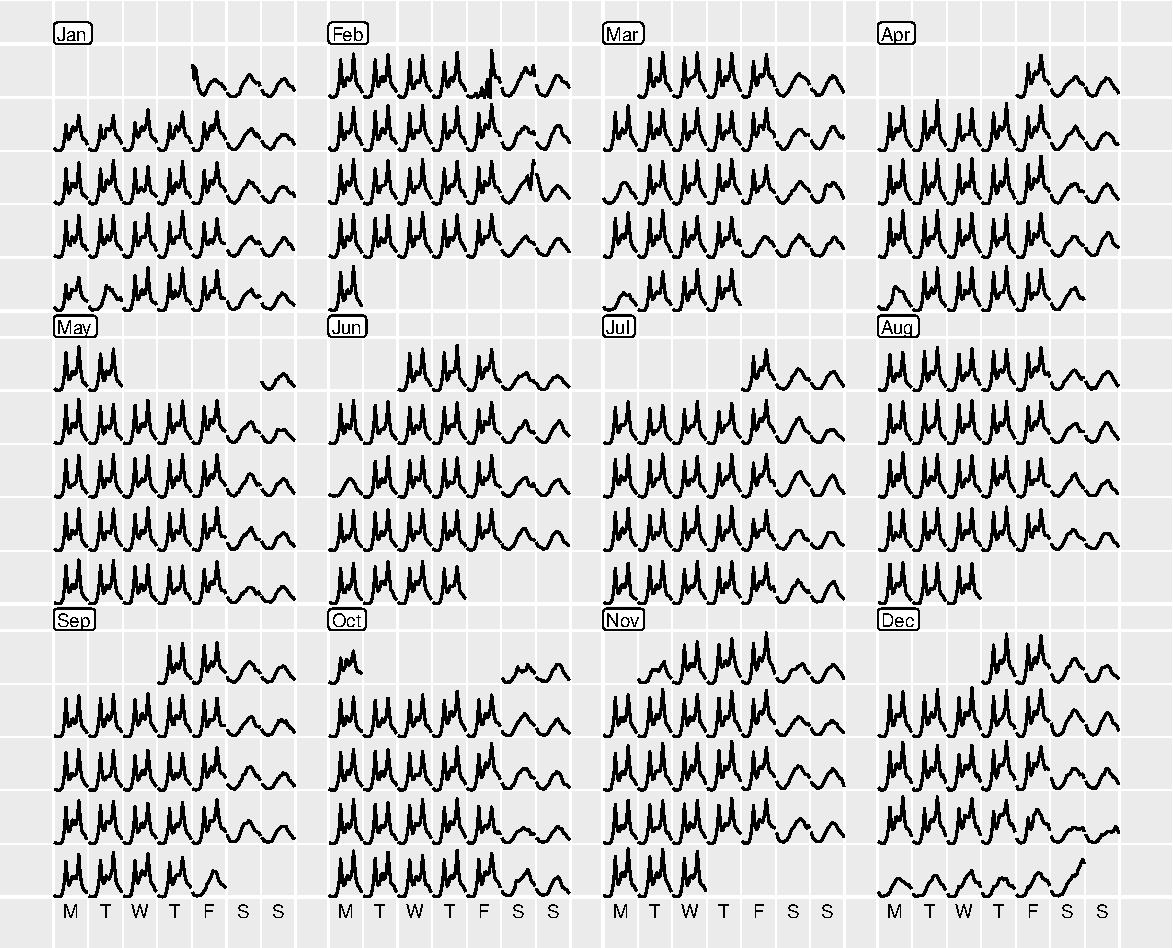
\includegraphics[width=\textwidth]{figure/flinders-2016-1} 

}

\caption[The calendar-based display of hourly foot
traffic at Flinders Street Station using line glyphs. The arrangement of
the data into a \(3 \times 4\) monthly grid represents all the traffic
in 2016. The disparities between week day and weekend along with public
holiday are immediately apparent.]{The calendar-based display of hourly foot
traffic at Flinders Street Station using line glyphs. The arrangement of
the data into a \(3 \times 4\) monthly grid represents all the traffic
in 2016. The disparities between week day and weekend along with public
holiday are immediately apparent.}\label{fig:flinders-2016}
\end{figure}
\end{CodeChunk}







The algorithm for constructing a calendar plot uses linear algebra,
similar to that used in the glyph map displays for spatio-temporal data
\citep{Wickham2012glyph}. To make a year long calendar, requires cells
for days, embedded in blocks corresponding to months, organized into a
grid layout for a year. Each month can be captured with 35 (5 \(\times\)
7) cells, where the top left is Monday of week 1, and the bottom right
is Sunday of week 5 by default. These cells provide a micro canvas on
which to plot the data. The first day of the month could be any of
Monday-Sunday, which is determined by the year of the calendar. Months
are of different length days, ranging from 28 to 31, and each month
could extend over six weeks but the convention in these months is to
wrap the last few days up to the top row of the block. The notation for
creating these cells is as follows:

\begin{itemize}
\tightlist
\item
  \(k = 1, \dots , 7\) is the day of the week that is the first day of
  the month.
\item
  \(d = 28, 29, 30\) or \(31\) representing the number of days in any
  month.
\item
  \((i, j)\) is the grid position where \(1 \le i \le 5\) is week within
  the month, \(1 \le j \le 7\), is day of the week.
\item
  \(g = k, \dots,(k+d)\) indexes the day in the month, inside the 35
  possible cells.
\end{itemize}

The grid position for any day in the month is given by

\begin{equation}
  \begin{aligned}
  i &= \lceil (g \mod 35) / 7\rceil, \\
  j &= g \mod 7. \label{eq:grid}
  \end{aligned}
\end{equation}

Figure \ref{fig:month-diagram} illustrates this \((i,j)\) layout for a
month where \(k=5\).

\begin{CodeChunk}
\begin{figure}

{\centering 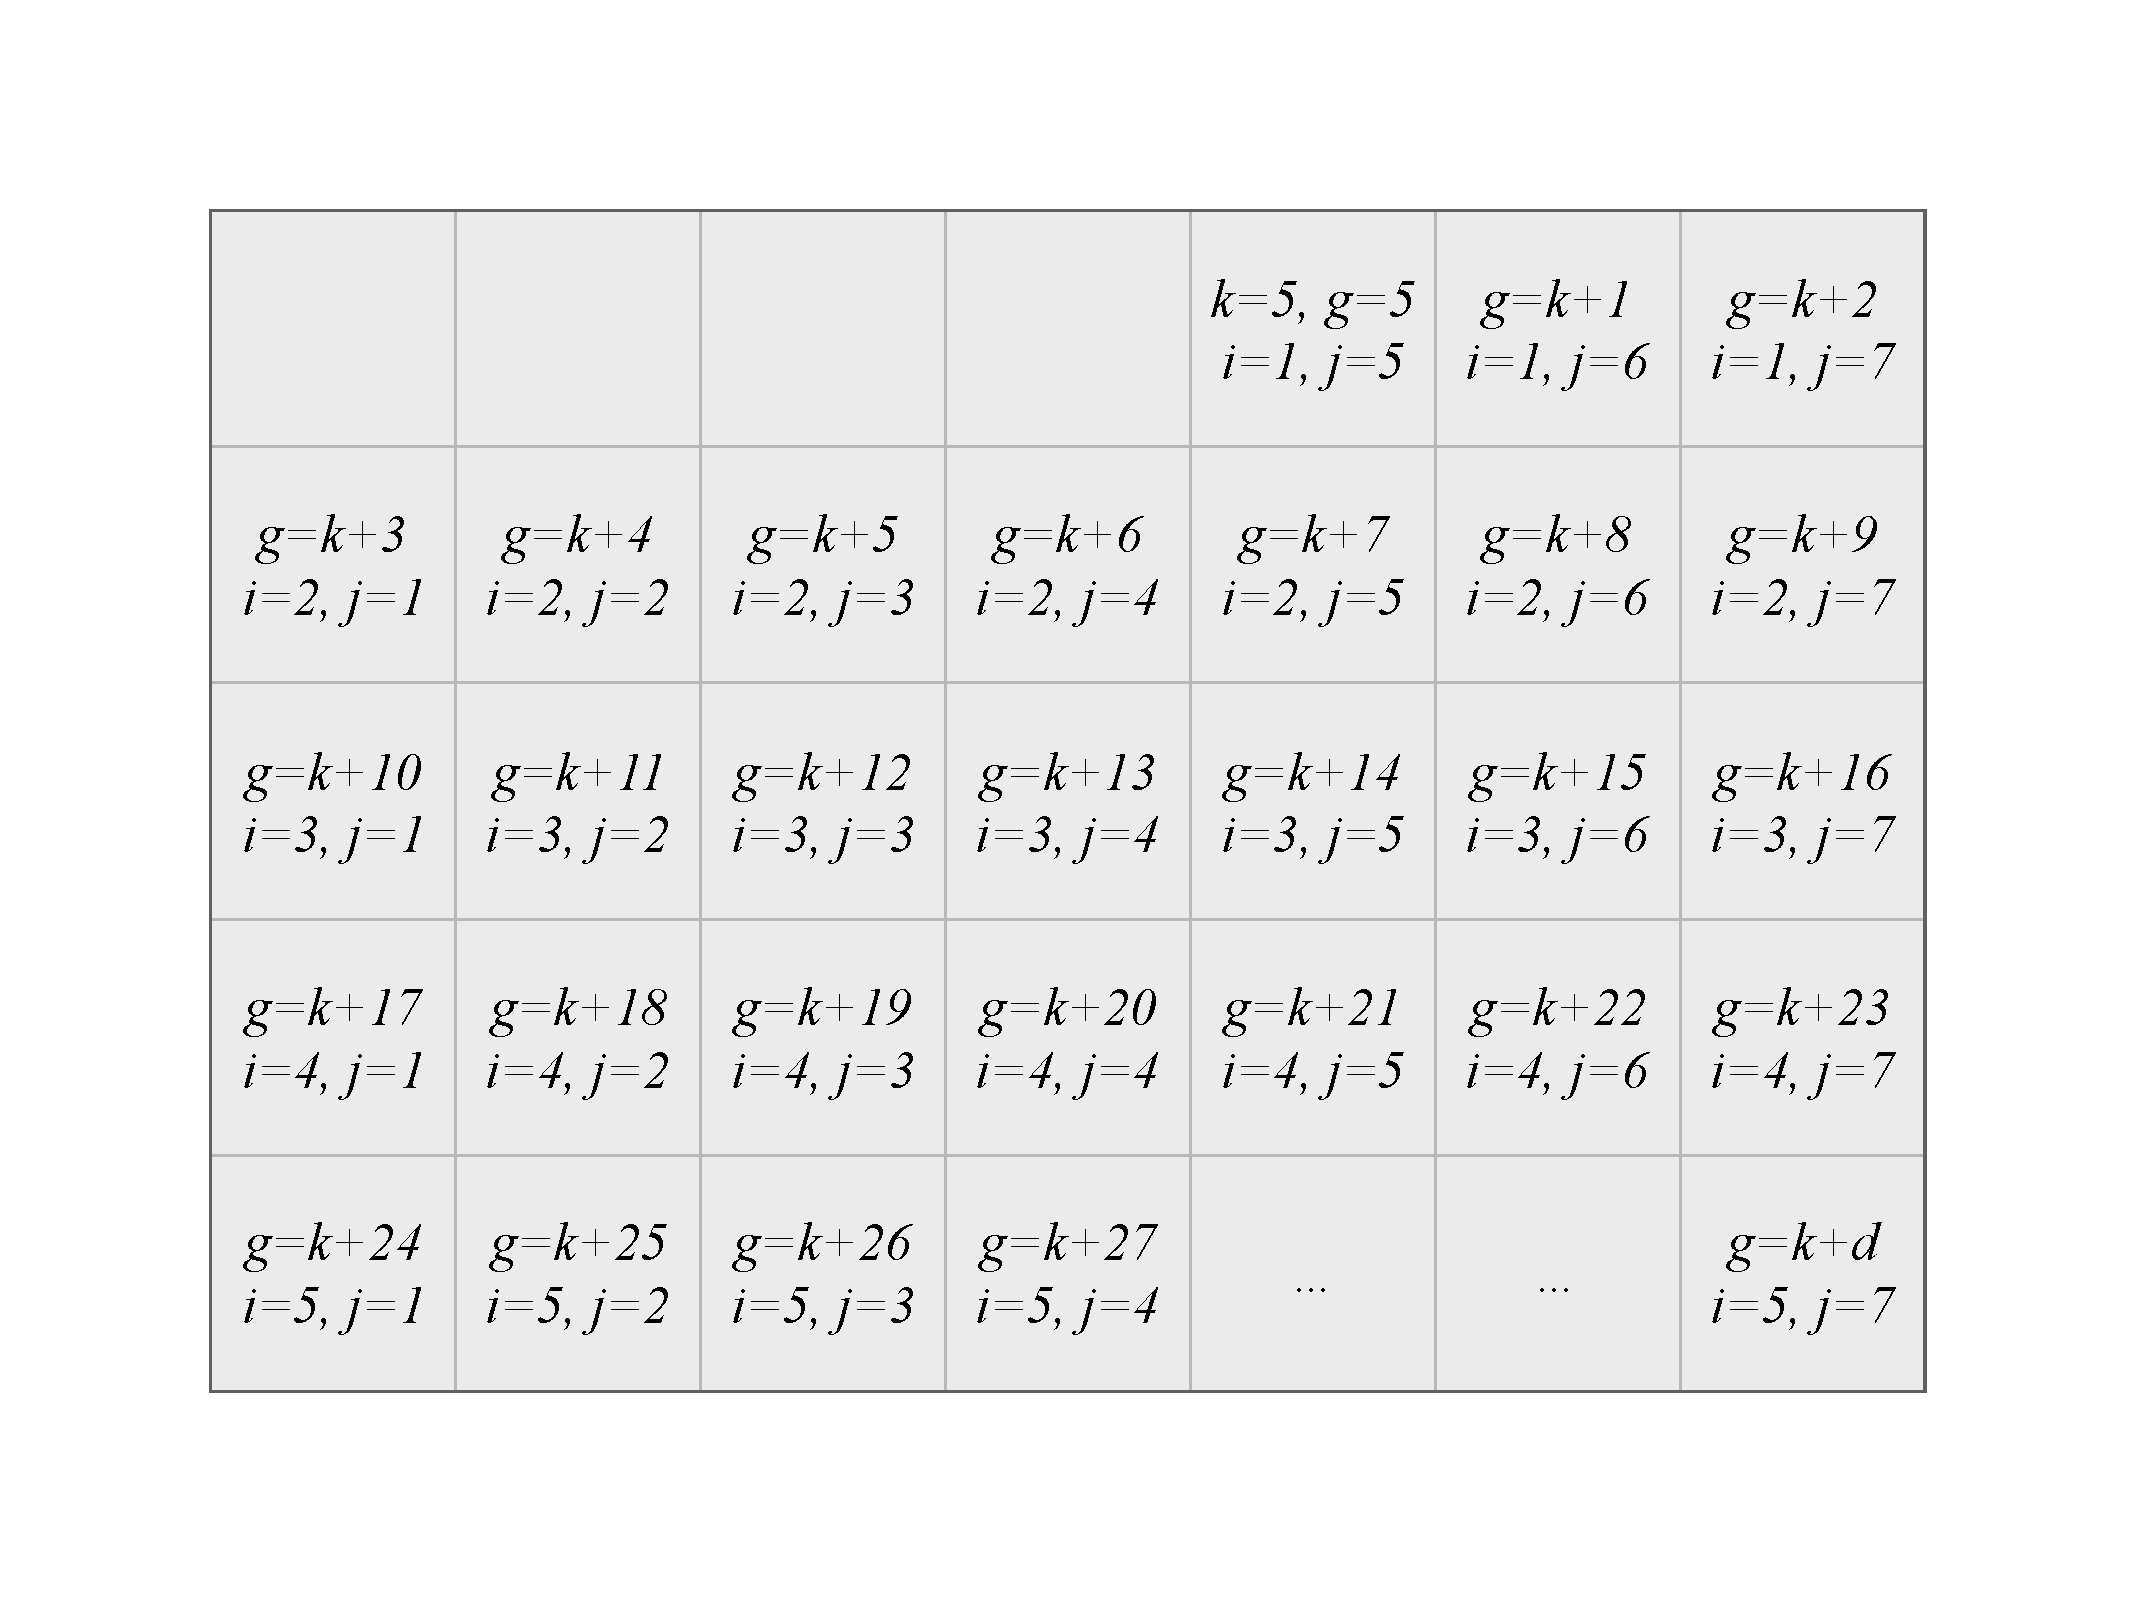
\includegraphics[width=360pt,height=250pt]{figure/month} 

}

\caption[Illustration of the indexing layout for cells in
a month.]{Illustration of the indexing layout for cells in
a month.}\label{fig:month-diagram}
\end{figure}
\end{CodeChunk}




To create the layout for a full year, \((m, n)\) denotes the position of
the month arranged in the plot, where \(1 \le m \le M\) and
\(1 \le n \le N\). Between each month requires some small amount of
white space, denoted by \(b\). Figure \ref{fig:year-diagram} illustrates
this layout where \(M = 3\) and \(N = 4\).

\begin{CodeChunk}
\begin{figure}

{\centering 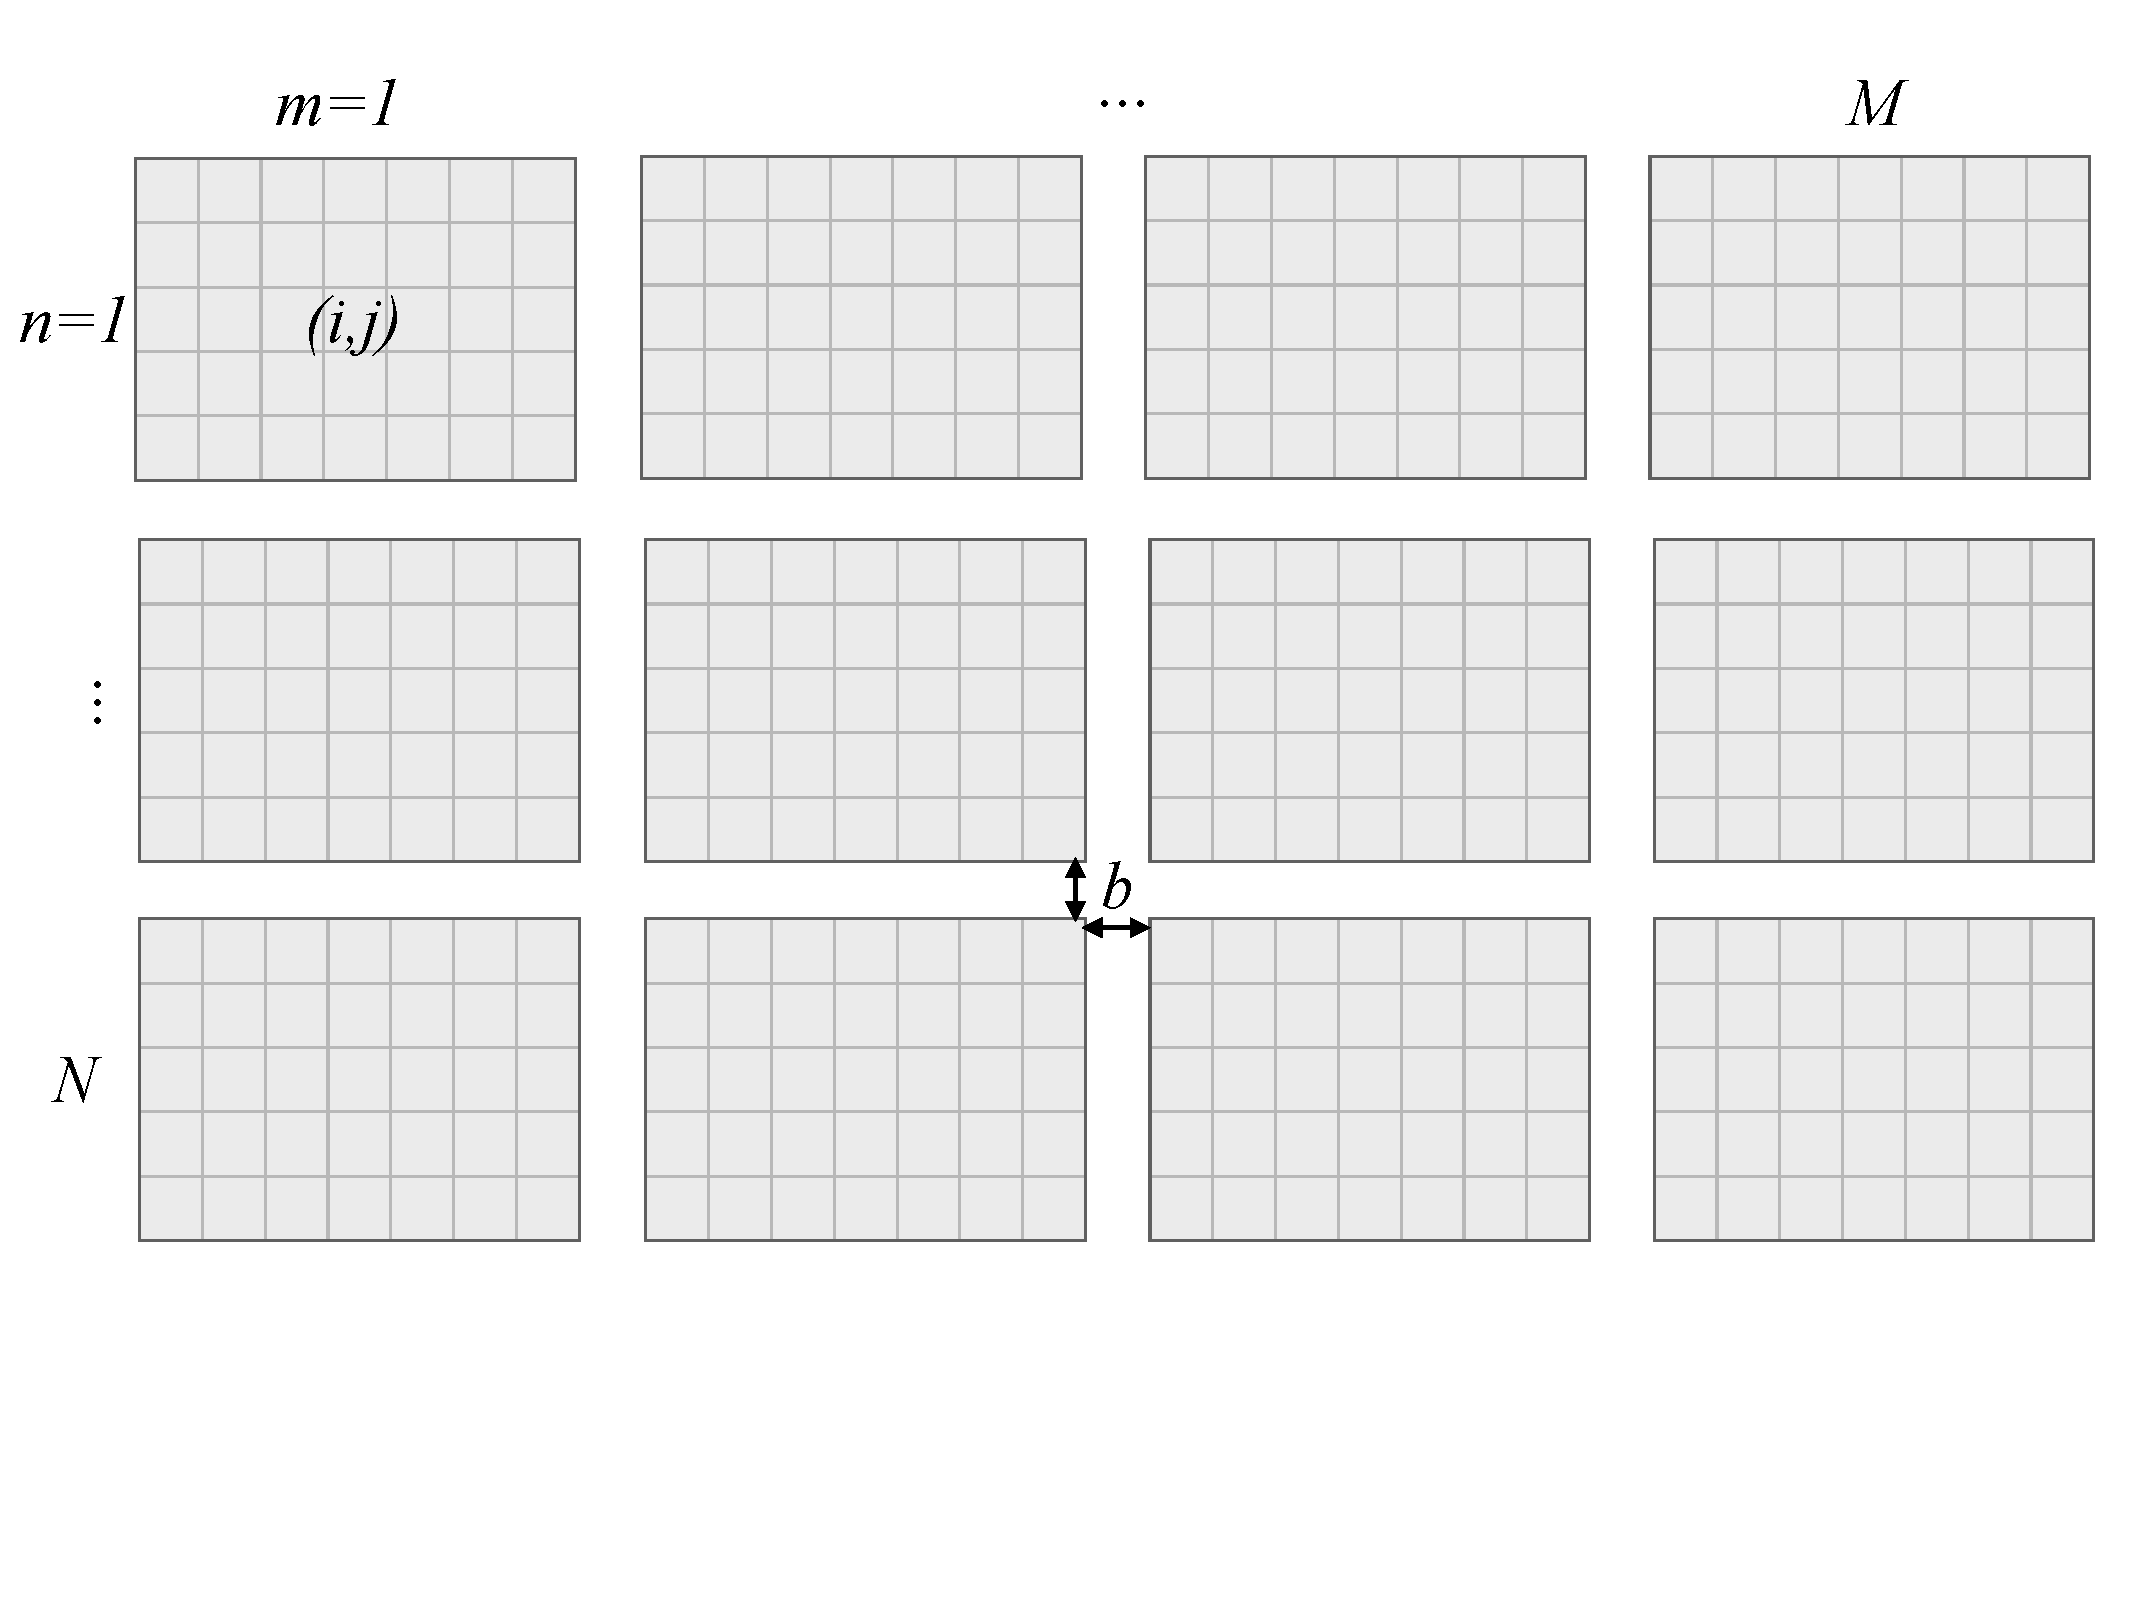
\includegraphics[width=360pt,height=250pt]{figure/year} 

}

\caption[Illustration of the indexing layout for months of
one year.]{Illustration of the indexing layout for months of
one year.}\label{fig:year-diagram}
\end{figure}
\end{CodeChunk}




Each cell forms a canvas on which to draw the data. Initialize the
canvas to have limits \([0, 1]\) both horizontally and vertically. For
the pedestrian sensor data, within each cell, hour is plotted
horizontally and count is plotted vertically. Each variable is scaled to
have values in \([0,1]\), using the minimum and maximum of all the data
values to be displayed, assuming fixed scales. Let \(h\) be the scaled
hour, and \(c\) the scaled count.

Then the final points for making the calendar line plots of the
pedestrian sensor data is given by:

\begin{equation}
  \begin{aligned}
  x &= j + (n - 1) \times 7 + (n - 1) \times b + h, \\
  y &= i - (m - 1) \times 5 - (m - 1) \times b + c. \label{eq:final}
  \end{aligned}
\end{equation}

Note that for the vertical direction, the top left is the starting point
of the grid (in Figure \ref{fig:month-diagram}) which is why subtraction
is performed. Within each cell, the starting position is the bottom
left.

In order to make calendar-based graphics more accessible and
informative, reference lines dividing each cell and block as well as
labels indicating week day and month are also computed before plotting
construction.

Regarding the monthly calendar, the major reference lines separate every
month panel and the minor ones separate every cell, represented by the
thick and thin lines in Figure \ref{fig:flinders-2016}, respectively.
The major reference lines are placed surrounding every month block: for
each \(m\), the vertical lines are determined by \(\min{(x)}\) and
\(\max{(x)}\); for each \(n\), the horizontal lines are given by
\(\min{(y)}\) and \(\max{(y)}\). The minor reference lines are only
placed on the left side of every cell: for each \(i\), the vertical
division is \(\min{(x)}\); for each \(j\), the horizontal is
\(\min{(y)}\).

The month labels located on the top left are obtained through
\((\min{(x)}, \max{(y)})\) for every \((m, n)\). The week day texts are
uniformly positioned on the bottom of the whole canvas, that is
\(\min{(y)}\), with the central position of a cell \(x / 2\) for each
\(j\).

\section{Options}\label{options}

\label{sec:opt}

There are several options provided for the \code{frame_calendar}
function to initialize and adjust the display of a calender plot:

\begin{verbatim}
frame_calendar(
  data, x, y, date, calendar = "monthly", dir = "h", sunday = FALSE, 
  nrow = NULL, ncol = NULL, polar = FALSE, scale = "fixed",
  width = 0.95, height = 0.95
)
\end{verbatim}

Assuming that tidy data \citep{wickham2014tidy} is the underlying data
structure, the parameter \code{x} takes a variable that will be mapped
to the horizontal axis and the parameter \code{y} mapped to the vertical
axis for plot construction. In Figure \ref{fig:flinders-2016}, for
example, the \code{x} is the variable specifying the time of the day,
and the \code{y} is the variable representing the hourly counts. The
\code{date} argument is given by the date variable that determines the
correct order of the calendar layout.

The algorithm can be extended to display data from a single month up to
a few years. The number of rows and columns in the layout can be
specified with the arguments \code{nrow} and \code{ncol}. If the one
would like to visualize data spanning over three years, for example,
\code{nrow = 3} and \code{ncol = 12} would be an appropriate choice when
assessing the differences of a given month across the years.

In Section \ref{sec:algorithm} we only illustrated that grids are laid
out horizontally. The vertical direction can be enabled by swapping
\(i\) and \(j\) in equation \eqref{eq:grid}, which occurs when the
argument \code{dir} is set to \code{"v"}. This benefits users who are
accustomed to calendars that are organized vertically, which is common
in some countries. Next we shall describe some of the arguments that
allow for alternate displays.

\subsection{Layouts}\label{layouts}

The algorithm described in Section \ref{sec:algorithm} is for the most
common calendar layout, the ``monthly'' calendar, but it can be
simplified to accommodate the other two types of calendar formats. One
is comprised of days of a week in columns and weeks of a year in rows,
and the other is days of a month in columns and months of a year in
rows, which we refer to as the ``weekly'' and ``daily'' calendar,
respectively. The layout to be used is controlled by the \code{calendar}
argument. The weekly calendar puts more emphasis on days of a week over
days of a year, whereas the daily calender does the opposite. The
monthly calender can be considered as the advanced variant of both
weekly and daily. Temporal patterns motivate which variant should be
employed. The weekly calendar is appropriate if most of the variation
can be characterised by days of the week. On the other hand, the daily
calendar should be used when there is a yearly effect but not a weekly
effect in the data. When both effects are present, the monthly calendar
would be a better choice.

\subsection{Polar transformation}\label{polar-transformation}

When \code{polar = TRUE}, the polar transformation is carried out on the
data. The computation is similar to the one described in
\citet{Wickham2012glyph}. Figure \ref{fig:flinders-polar} shows star
plots embedded in the monthly calendar layout, which is equivalent to
Figure \ref{fig:flinders-2016} placed in polar coordinates.

\begin{CodeChunk}
\begin{figure}

{\centering 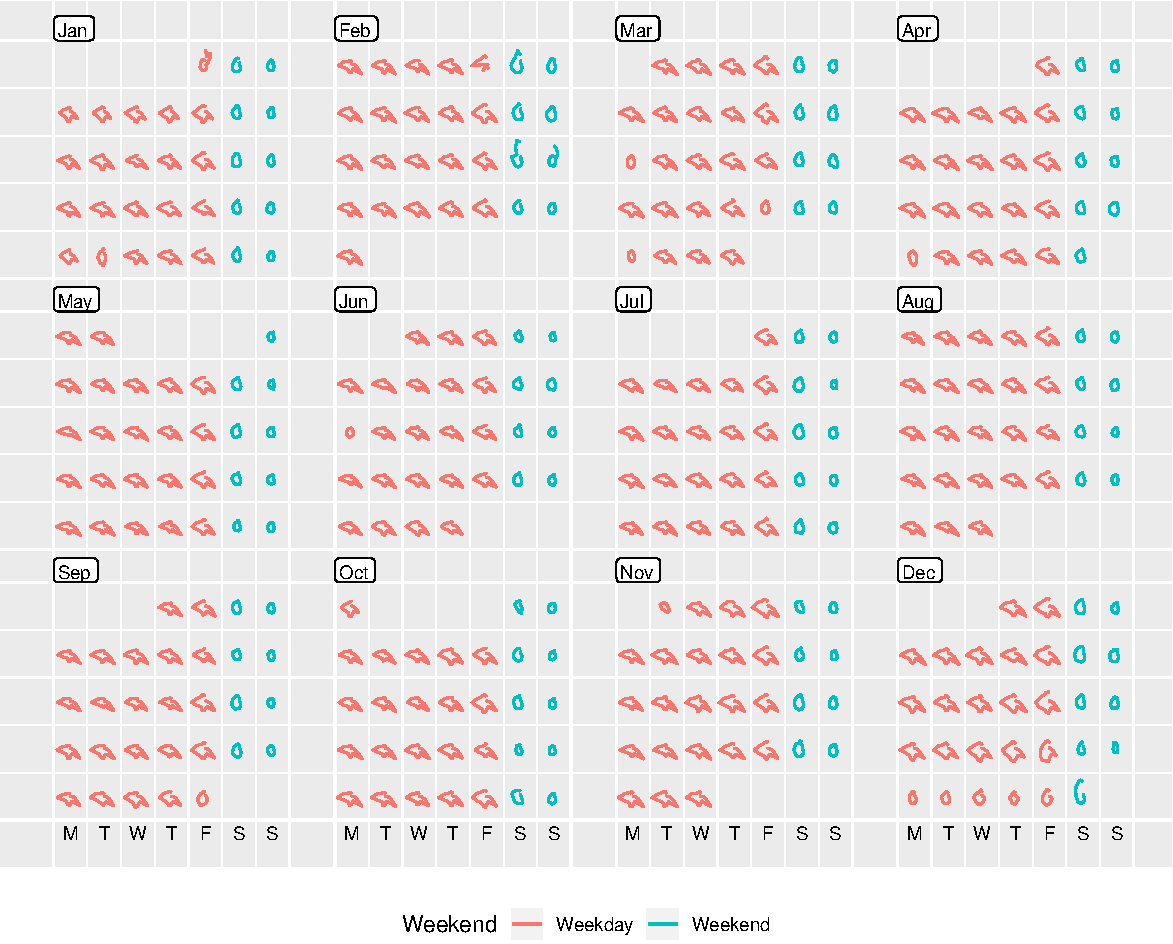
\includegraphics[width=\textwidth]{figure/flinders-polar-1} 

}

\caption[Figure \ref{fig:flinders-2016} in circular
layout, which is referred to as star plots. The daily periodicity on
work days are clearly visible.]{Figure \ref{fig:flinders-2016} in circular
layout, which is referred to as star plots. The daily periodicity on
work days are clearly visible.}\label{fig:flinders-polar}
\end{figure}
\end{CodeChunk}





\subsection{Scales}\label{scales}

Section \ref{sec:algorithm} discusses the implementation applied to a
fixed scale, which uses the range over all data values. The \code{scale}
argument controls the scaling of the display. The fixed scale
(\code{fixed}) is the default, meaning that the data values in all
positions are scaled. The remaining options include: free scale within
each cell (\code{free}), cells derived from the same day of the week
(\code{free_wday}), or cells from the same day of the month
(\code{free_mday}). The scaling allows for the comparisons of absolute
or relative values, and the emphasis of different temporal variations.

Grouping the cells based on the corresponding time period gives rise to
the different scales. For example, the minimums and maximums obtained
from each cell produce a local scale. The overall variation gives way to
the individual shape. Figure \ref{fig:flinders-free} is an example of
plotting line charts scaled locally using \code{scale = "free"}. The
daily variation is more distinctive compared to Figure
\ref{fig:flinders-2016}.

The \code{free_wday} suggests that the scales are common for a given
week day across all weeks, but different for each week days within a
week. In other words, the same value within a given Monday, for example,
corresponds to the same position across all Mondays but the different
position in other week days. Similarly, the \code{free_mday} suggests
free scaling for any day within a given month. The scaling choices
combined with the calendar layouts offers a number of varieties to
construct the plot.

\begin{CodeChunk}
\begin{figure}

{\centering 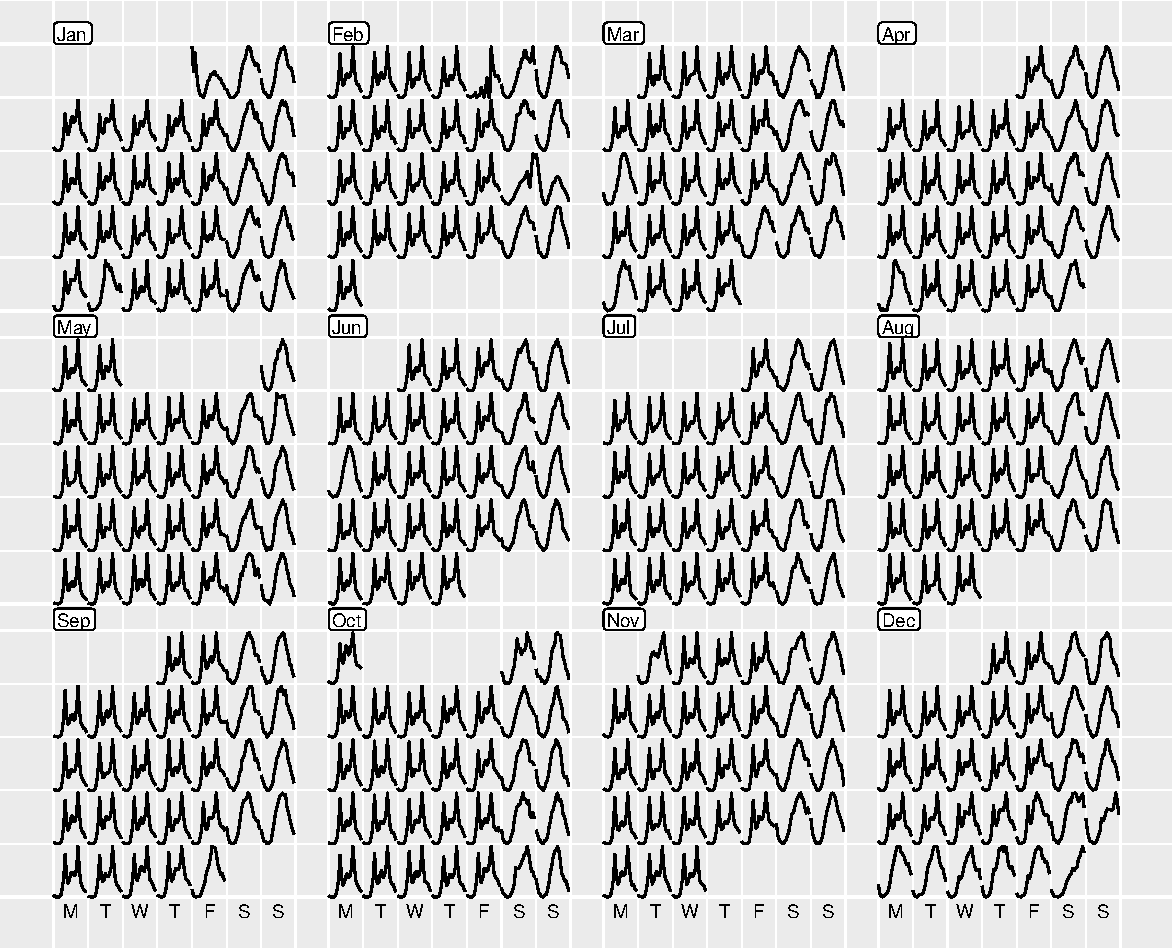
\includegraphics[width=\textwidth]{figure/flinders-free-1} 

}

\caption[Line glyphs on the calendar format showing
hourly foot traffic at Flinders Street Station, scaled over all the
days. The individual shape on a single day becomes more distinctive,
however it is more difficult to compare the size of peaks between days.]{Line glyphs on the calendar format showing
hourly foot traffic at Flinders Street Station, scaled over all the
days. The individual shape on a single day becomes more distinctive,
however it is more difficult to compare the size of peaks between days.}\label{fig:flinders-free}
\end{figure}
\end{CodeChunk}






\section{Variations}\label{variations}

\label{sec:examples}

\subsection{Overlaying and faceting
subsets}\label{overlaying-and-faceting-subsets}

The comparison of one sensor to another adds additional insights to the
dataset, which is often done with an overlaying plot such as Figure
\ref{fig:overlay}. For instance, the dominant patterns that occurred at
Flinders Street and Flagstaff train stations are driven by the commuters
on work days; however, Flinders Street Station has higher pedestrian
counts during the weekends and public holidays. This suggests that
Flagstaff Station limits its functionality on non-work days, but various
activities take place around the Flinders Street Station other than
commuting. Figure \ref{fig:overlay} also shows that State Library
follows a similar temporal trend as Flinders Street Station on non-work
days. The nighttime events, such as White Night and New Year's Eve, have
barely affected the operation of Flagstaff Station but heavily affected
the incoming and outgoing traffic to Flinders Street Station and State
Library.

\begin{CodeChunk}
\begin{figure}

{\centering 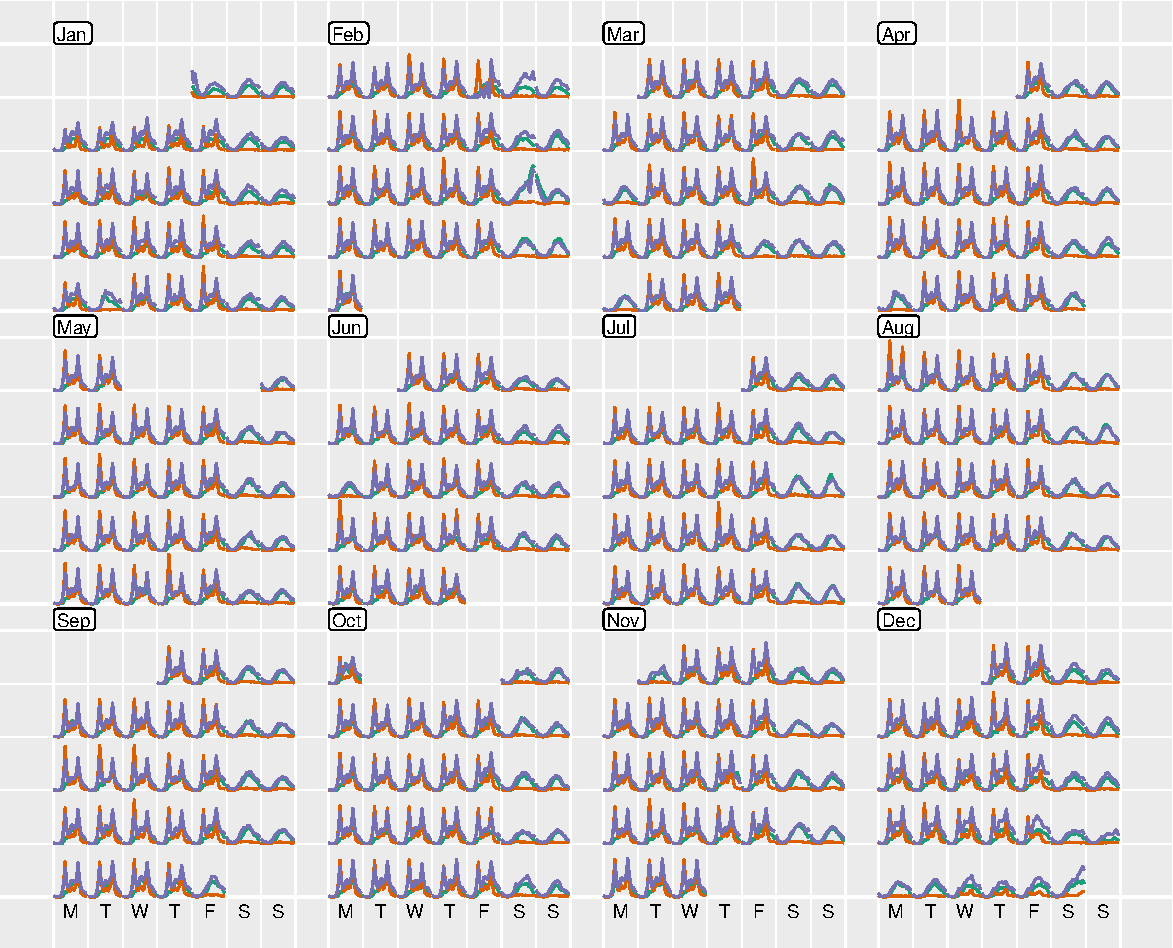
\includegraphics[width=\textwidth]{figure/overlay-1} 

}

\caption[Overlaying line graphs of the 3 sensors in the monthly
calendar. Flagstaff station is not as busy as the other two on non-work
days.]{Overlaying line graphs of the 3 sensors in the monthly
calendar. Flagstaff station is not as busy as the other two on non-work
days.}\label{fig:overlay}
\end{figure}
\end{CodeChunk}





To avoid the overlapping problem, the calendar layout can be embedded
into a series of subplots for the different sensors. Figure
\ref{fig:facet} presents the idea of faceting calendar plots. This
allows comparing the overall structure between sensors, while
emphasising individual sensor variation.

\begin{CodeChunk}
\begin{figure}

{\centering 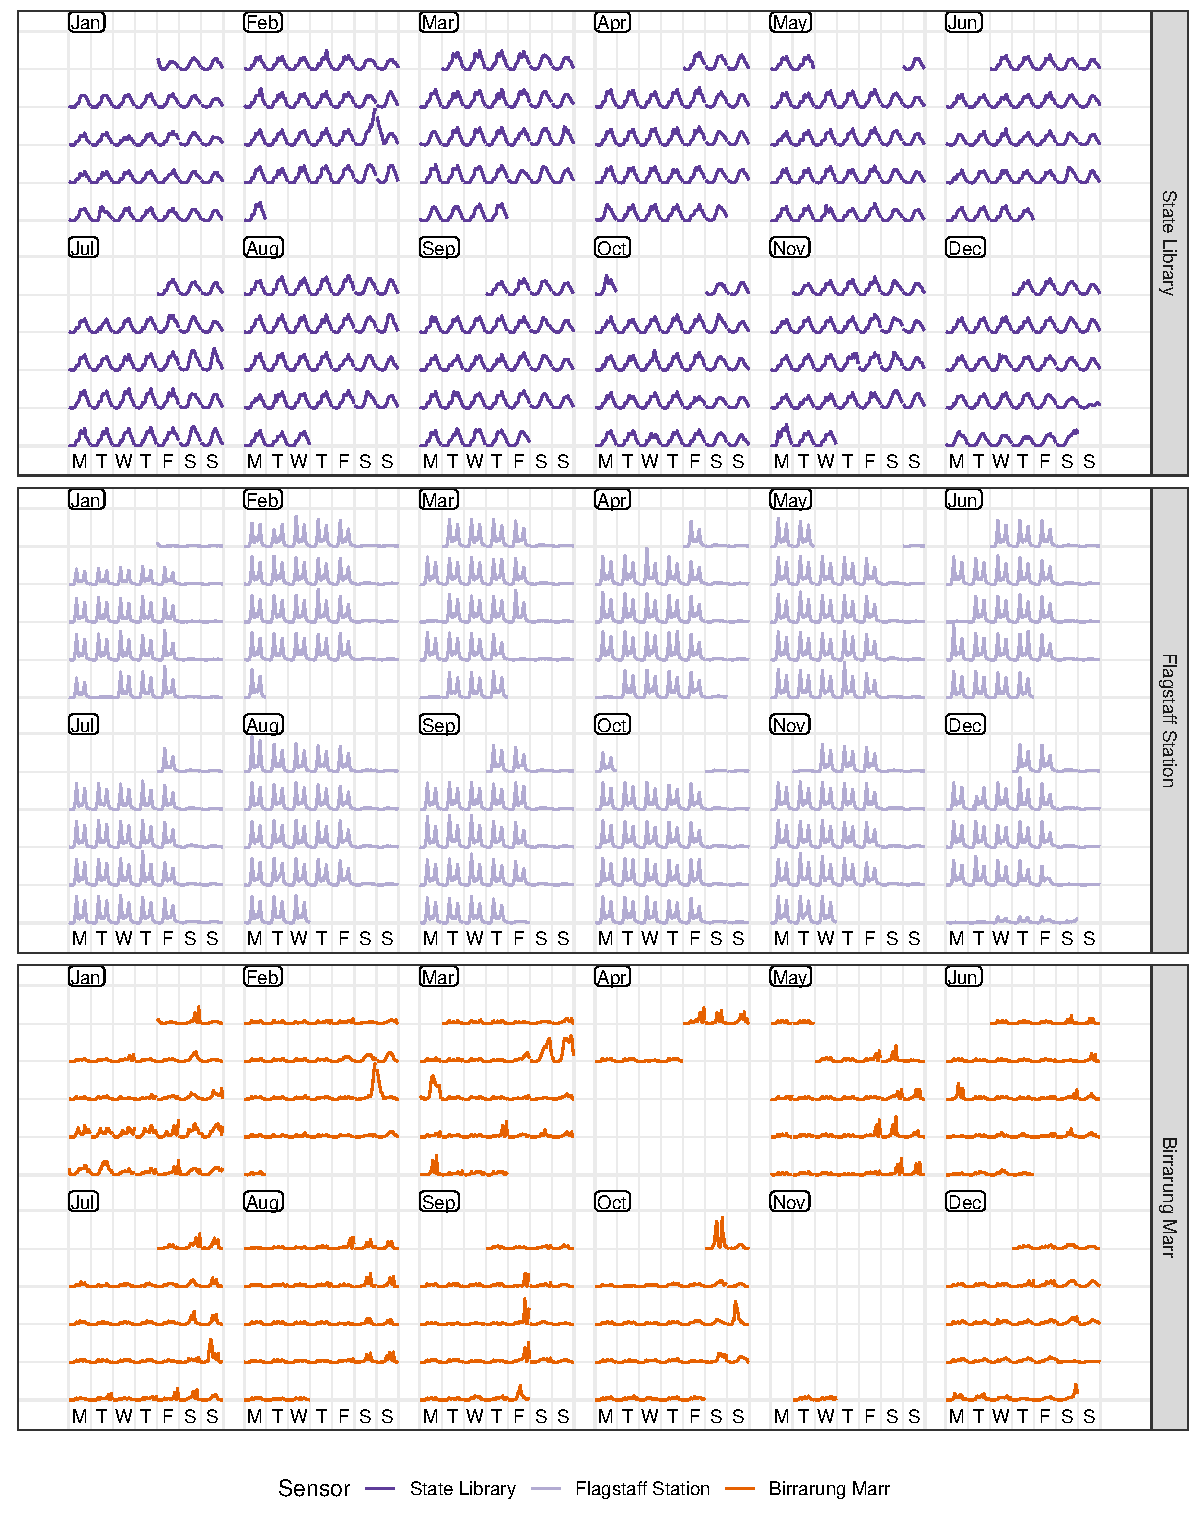
\includegraphics[width=\textwidth]{figure/facet-1} 

}

\caption[Line charts, embedded in the \(6 \times 2\) monthly
calendar, coloured and faceted by the 3 sensors. The variations of an
individual sensor are emphasised, and the shapes can be compared across
the cells and sensors.]{Line charts, embedded in the \(6 \times 2\) monthly
calendar, coloured and faceted by the 3 sensors. The variations of an
individual sensor are emphasised, and the shapes can be compared across
the cells and sensors.}\label{fig:facet}
\end{figure}
\end{CodeChunk}






\subsection{Different types of plots}\label{different-types-of-plots}

The \code{frame_calendar} function does not constrain itself to mapping
only the temporal variable to the \code{x} argument. Figure
\ref{fig:scatterplot} shows a lag scatterplot at Flinders Street
Station, where the current hourly count is assigned to the \code{x}
argument and the lagged hourly count to the \code{y} argument. This
figure is organized in the daily calendar layout. It provides a visual
tool for identifying repeating patterns. Figure \ref{fig:scatterplot}
indicates two separate paths in the work-day glyphs, suggesting that an
hour of a work day with many pedestrians is likely to be followed in the
next hour with either greater or fewer numbers of pedestrians. However,
this pattern is absent on non-work days. There is a bimodality on work
days while there is unimodality on the rest of the days, which is also
supported by Figure \ref{fig:flinders-2016}.

\begin{CodeChunk}
\begin{figure}

{\centering 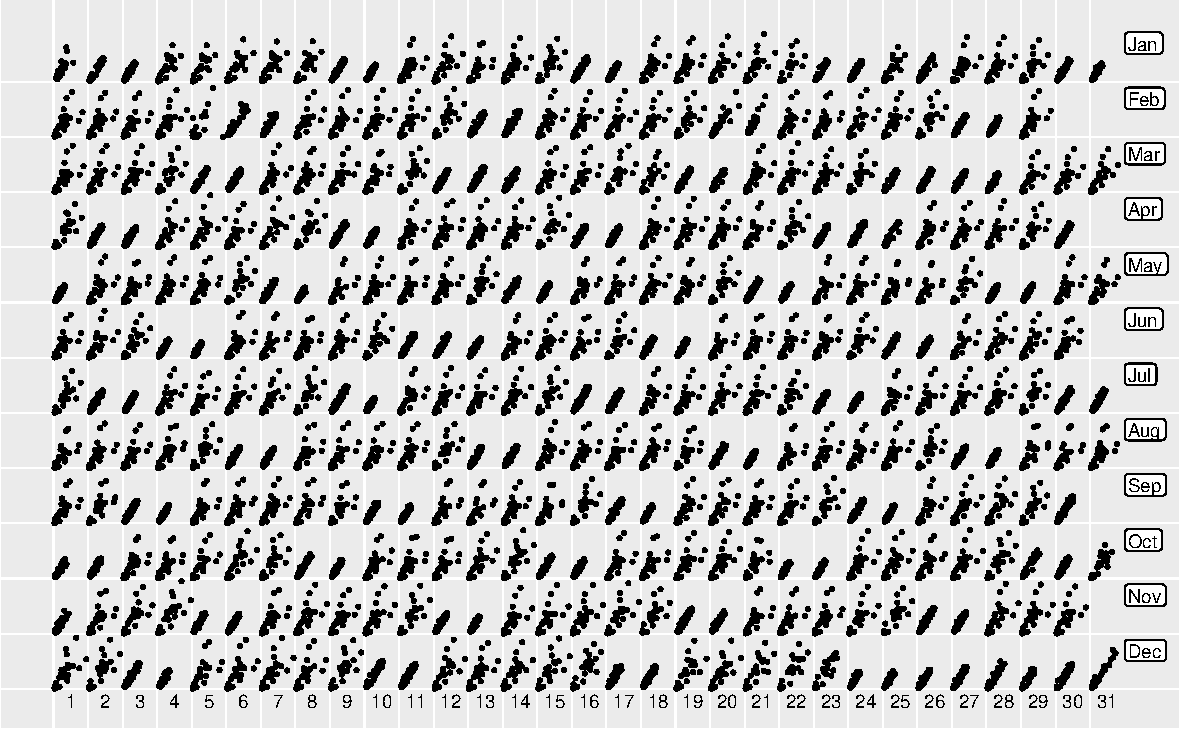
\includegraphics[width=\textwidth]{figure/scatterplot-1} 

}

\caption[Lag scatterplot in the daily calendar layout.
Previous hour's count is plotted against each hour's count at Flinders
Street Station to demonstrate the autocorrelation at lag 1. The
correlation between them is more consistent on non-work days than work
days.]{Lag scatterplot in the daily calendar layout.
Previous hour's count is plotted against each hour's count at Flinders
Street Station to demonstrate the autocorrelation at lag 1. The
correlation between them is more consistent on non-work days than work
days.}\label{fig:scatterplot}
\end{figure}
\end{CodeChunk}







The newly computed coordinates can work with more complicated plots,
such as the boxplot. Figure \ref{fig:boxplot} uses the loess smooth line
superimposed on side-by-side boxplots. It shows the distribution of
hourly counts across all 43 sensors at a given time point during
December. In general, bimodality features on work days whereas
unimodality features on the rest of the days. The last week of December
is the holiday season: people are off work on the day before Christmas,
go shopping on the Boxing day, and stay out for the fireworks on New
Year's Eve.

\begin{CodeChunk}
\begin{figure}

{\centering 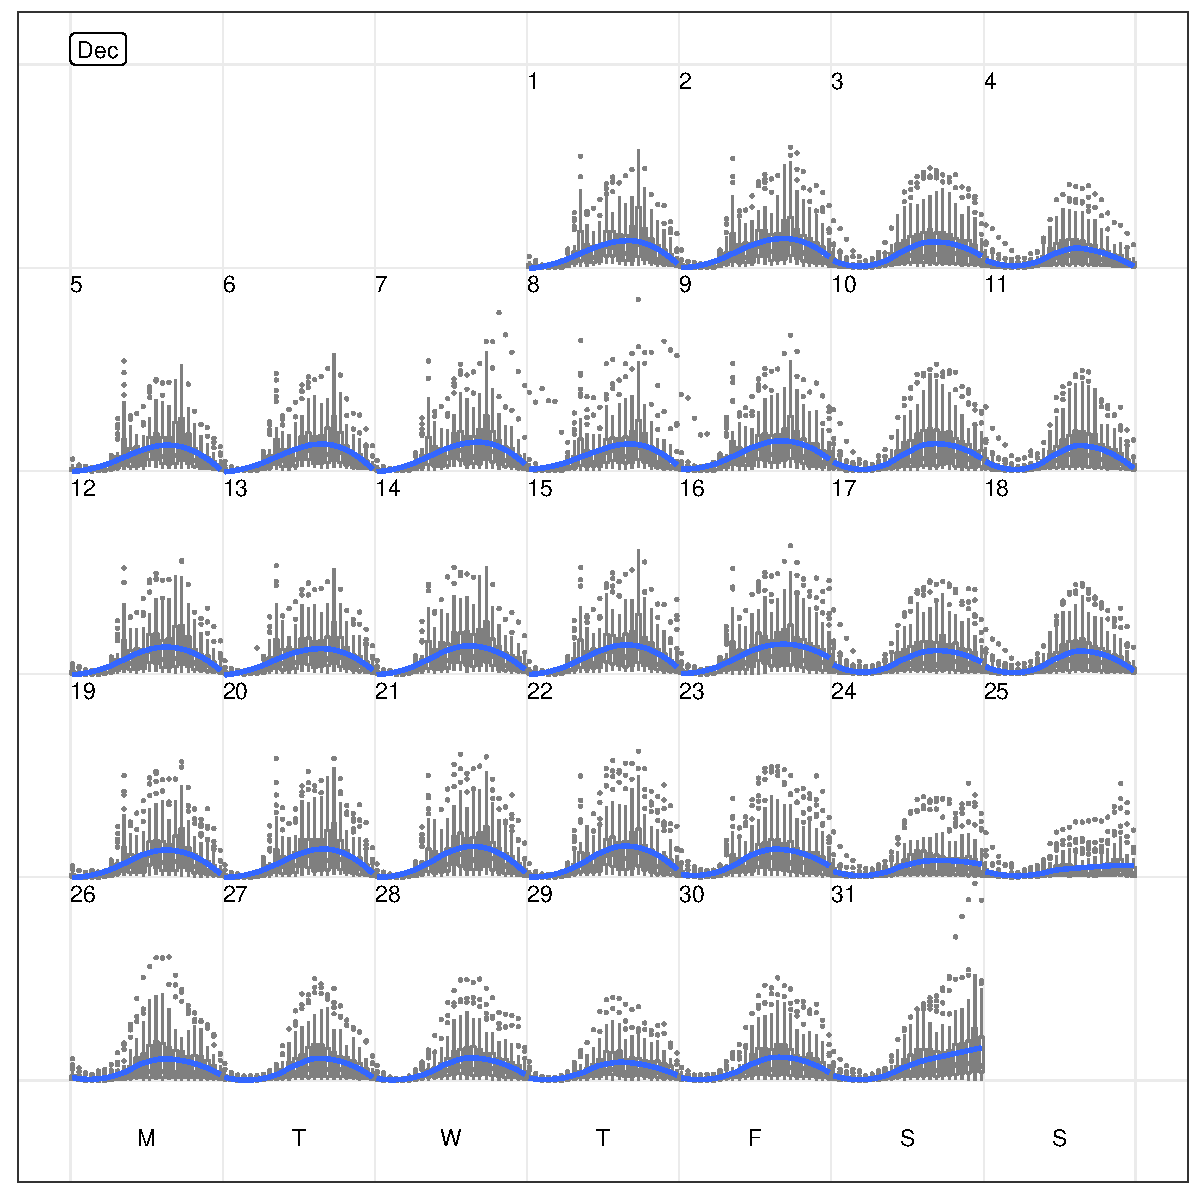
\includegraphics[width=\textwidth]{figure/boxplot-1} 

}

\caption[Side-by-side boxplot of hourly counts across all the
43 sensors in December of 2016, with the superimposing loess smooth line
for each day. It shows the hourly distribution in the city as a whole.
There is one sensor attracting a larger number of people on New Year's
Eve than the rest.]{Side-by-side boxplot of hourly counts across all the
43 sensors in December of 2016, with the superimposing loess smooth line
for each day. It shows the hourly distribution in the city as a whole.
There is one sensor attracting a larger number of people on New Year's
Eve than the rest.}\label{fig:boxplot}
\end{figure}
\end{CodeChunk}







These calendar layouts, especially the monthly calendar, become widely
used in society. We offer languages other than English for text
labelling. Figure \ref{fig:chn} shows the same plot as Figure
\ref{fig:boxplot} labelled using simplified Chinese characters.

\begin{CodeChunk}
\begin{figure}

{\centering 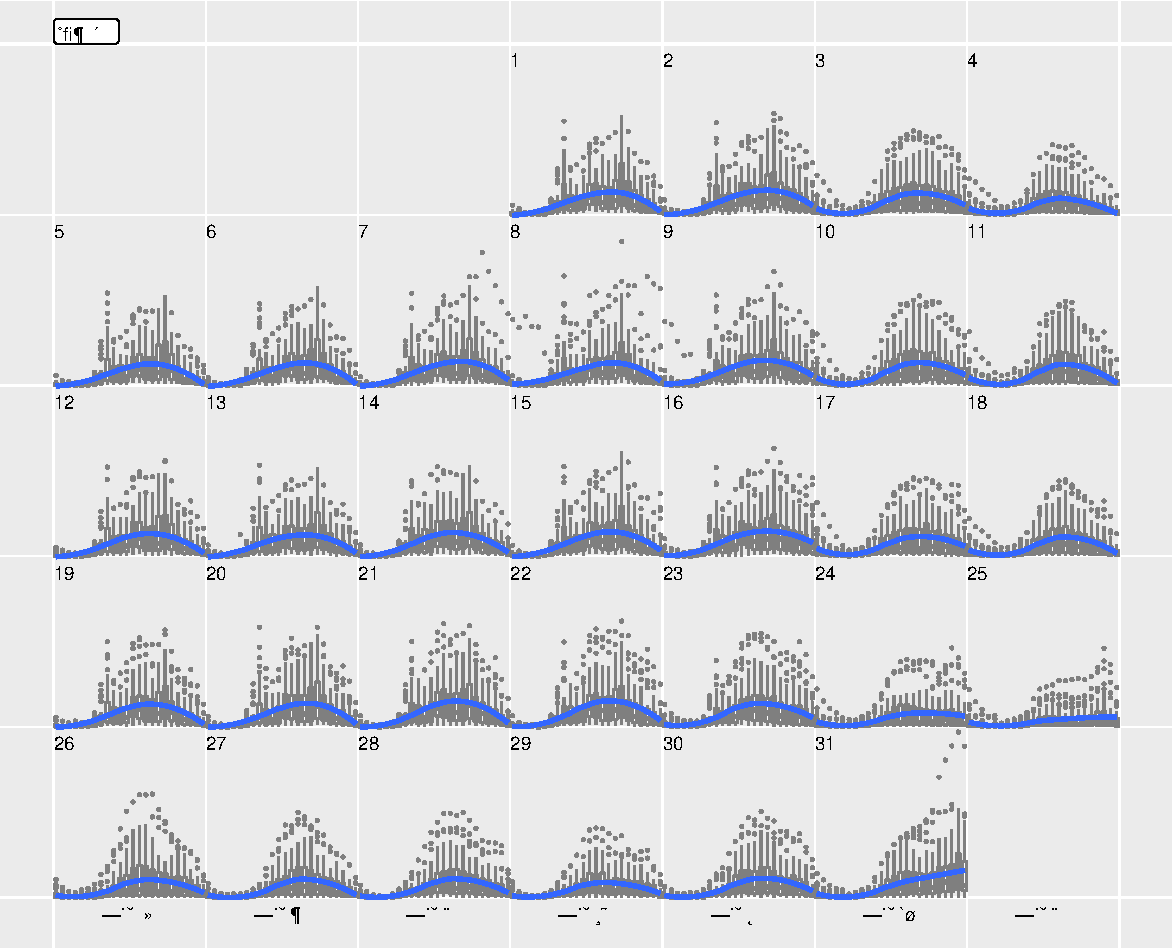
\includegraphics[width=\textwidth]{figure/chn-1} 

}

\caption[The same side-by-side boxplot as Figure \ref{fig:boxplot},
but with the month and week day labels in Chinese. It demonstrates the
natural support for languages other than English.]{The same side-by-side boxplot as Figure \ref{fig:boxplot},
but with the month and week day labels in Chinese. It demonstrates the
natural support for languages other than English.}\label{fig:chn}
\end{figure}
\end{CodeChunk}





\section{Discussion}\label{discussion}

\label{sec:discussion}

The calendar-based visualization provides data plots in the familiar
format of an everyday tool. Special events for the region, like Anzac
Day in Australia, or Thanksgiving Day in the USA, more easily pop out to
the viewer as public holidays, rather than a typical work day.

This sort of layout may be useful for studying consumer trends, or human
behavior, like the pedestrian patterns. It may not work so well for
physical patterns like temperature, which are not typically affected by
human activity.

\bibliography{packages.bib,references.bib}


\end{document}

